\chapter{Методы численного моделирования}
\label{ch:methods}


\section{Обзор различных подходов}

 \subsection{Полный перебор} 
 
При небольшом размере системы (короткие цепочки и малое число спинов) можно перебрать все возможные конфигурации и использовать весь набор для подсчета физических величин \cite{Schram_2011}.  Этот метод даёт точные результаты  для дискретных спинов. В случае непрерывных спиновых переменных, можно использовать полный перебор БСП фиксированной длины, генерируя большое количество спиновых конфигураций для каждого, что позволит также получить достаточно точные результаты для получения средних. 

Метод полного перебора крайне плохо масштабируется  из-за экспоненциального роста числа состояний и не может применяться для моделирования длинных полимерных цепочек. 

Мы используем метод полного перебора на коротких цепочках для верификации реализованного метода Монте-Карло по Марковской цепи \ref{MCMC}. 

 %  Аналитические методы или приближенные 


%\section{Метод Монте-Карло по Марковской цепи}
 
 \subsection{Метод Монте-Карло} 
Методы Монте-Карло являются универсальным методом для моделирования систем с большим  числом степеней свободы, в которых перебор невозможен \cite{Landau_Binder_2021, Barkema}.

Базовый метод Монте-Карло использует случайное выборочное усреднение: нужную величину представляют как математическое ожидание и оценивают средним по независимым случайным выборкам.  

При моделировании сложных систем, как правило, получение независимой выборки затруднено.
 Так, при моделировании БСП число конфигураций растет экспоненциально как $\mu^N$ \cite{Rensburg}, где  $\mu \approx  4.684039931(27) $ для случая $d=3$ \cite{clisby2007self},  а число возможных шагов для траектории случайного блуждания на кубической решетке  $(2d)^N = 6^N$. Вероятность получить БСП при случайной генерации 
 экспоненциально мала для больших цепочек $N$  (так как убывает с $(\mu/6)^N$). 
 
 \subsection{ Метод Монте-Карло по Марковской цепи }
  \label{MCMC_description_general}
 
Для эффективного моделирования сложных систем одним из универсальных семейств методов являются методы Марковских цепей Монте‑Карло (MCMC ).   Суть методов заключается в  формировании цепочки состояний, переходы в которой заданы так, чтобы её стационарное распределение совпадало с целевым. Такие методы позволяют эффективно изучать системы, где состояния распределены согласно распределению  Больцмана-Гиббса  \eqref{Zcanonical}.

 % распределены согласно распределению   ---  плохо 

Средние наблюдаемых, полученные при траектории Марковской цепи сходятся к истинным ансамблевым средним при выполнении двух условий: эргодичности и детального баланса.  

Эргодичность подразумевает, что любое состояние системы можно достичь из любого другого за конечное число шагов с ненулевой вероятностью. Условие эргодичности гарантирует, что алгоритм  со временем посещает всё конфигурационное пространство.


Детальный баланс в физике означает, что в равновесии каждый переход (новое состояние) компенсируется обратным (поток переходов между любыми двумя состояниями уравновешен).  Условие детального баланса  обеспечивает сходимость к равновесному распределению и выглядит следующим образом:

 \begin{equation}
	\label{detailedbalance}
	p_{u_0} P(u_0 \rightarrow u_{new} ) = p_{u_{new}} P( u_{new} \rightarrow u_0),
\end{equation}
где $P(u_0\rightarrow u_{new} )$ --- вероятность перехода из состояния $u_0$ в состояние  $u_{new}$. Здесь $p_{u_0},p_{u_{new}}$ --- стационарная вероятность нахождения в состоянии  $p_{u_0} = e ^{-H(u_0)}/Z $ из распределения Гиббса-Больцмана.   
  
%Условие детального баланса обеспечивает сходимость к равновесному распределению.


Один из самых известных методов Монте-Карло по Марковской цепи --- метод Метрополиса  \cite{MetropolisOriginal}. Суть метода: генерируется новое состояние $u_{new}$, которое принимается с вероятностью  $P_{accept} = \min (1, e^{ - \Delta E})$, где $\Delta E$ ---  разность энергий между новым и текущим состоянием.  % Такой подход обеспечивает сходимость к равновесному распределению при выполнении условия детального баланса.




\section{Метод Монте-Карло по Марковской цепи: 3  шага}
\label{MCMC}

В этом исследовании используется метод Монте-Карло на основе Марковских цепей для моделей, объединяющих спиновые переменные и динамическую геометрию.  Вдохновение, полученное  из книги  \cite{Barkema} позволило адаптировать классические алгоритмы к поставленным задачам. 



\subsection{Метрополис (змееподобный алгоритм)}
\label{subsection:snake}

\begin{figure}
	\centering
	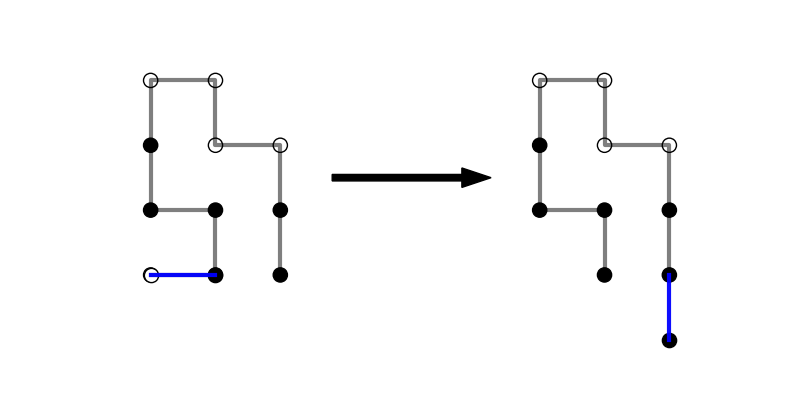
\includegraphics[width=0.45\textwidth]{images/snakeupdate.png}
	\caption{Пример "змееподобного алгоритма".}
	\label{fig:snakeupdate}
\end{figure}  

Для моделирования спиновых систем на динамической геометрии мы используем модифицированный "змееподобный алгоритм" (slithering snake algorithm/Reptation algorithm) \cite{Binder_Sokal_chapter}, основанный на методе Метрополиса  \cite{MetropolisOriginal}.  Это классический метод, применяемый для моделирования БСП в каноническом ансамбле. Генерация нового состояния - это  следующие шаги: 1) Выбирается один из концов цепочки; 2)  Удаляется выбранный конец в шаге 1; 3) добавляет новый узел блуждания в случайном направлении на другом конце \ref{fig:snakeupdate}.   

В нашей работе рассматриваются системы, где спиновые состояния динамичные, поэтому при генерации нового состояния алгоритмом мы также  генерируем случайное спиновое значение для нового мономера. Общая схема этого алгоритма в наших реализациях выглядит так:

 \begin{enumerate}
\item Фиксируется  текущее состояние системы  $u_0$. 

\item  Выбирается один из концов цепочки, который предполагается для удаления. 

\item  Выбирается случайным образом из равномерного   распределения одно из  $2 \times d$ направлений ($d $ - размерность пространства). В это направление должен добавиться новый мономер на другом конце цепочки. 

\item Проверяется условие на самопересечение: в цепочке не должно быть узла в новой координате. Если условие на отсутствие самопересечений не выполняется, то новое состояние отклоняется и генерация начинается с шага 1.

 \item Удаляется выбранный конец цепочки в шаге 2. Добавляется новый мономер в координату, определенные на шаге 3. 

 \item Для нового мономера БСП генерируется  переменная из спинового пространства. Генерация нового состояния $u_{new}$  завершается. 
 
 
 \item  Новое сгенерированное состояние  $u_{new}$ принимается по правилу Метрополиса:
 \begin{equation}
 	\label{accratios}
 	A(u_0  \rightarrow u_{new} ) =  
 	\begin{cases}
 		e^{-J(E_{u_{new}}-E_{u_0})}, & \text{if $E_{u_{new}}-E_{u_0}>0$;}\\
 		1, & \text{иначе}.
 	\end{cases} 
  \end{equation}


\end{enumerate}

  \textbf{Детальный баланс}. 

Для генерации состояний системы согласно распределению Больцмана-Гиббса, вводится коэффициент принятия перехода $A(u_0  \rightarrow u_{new} )$: 
\begin{equation*}
	P(u_0  \rightarrow u_{new} ) = g(u_0  \rightarrow u_{new} ) A(u_0  \rightarrow u_{new} ),
\end{equation*}

где $g(u_0  \rightarrow u_{new} )$ вероятность  сгенерировать алгоритмом  состояние $u_{new} $ из состояния  $u_0$. 
 Обозначение $ A(u_0  \rightarrow u_{new} )$ --- вероятность алгоритмом принять новое состояние $u_{new} $ и изменить состояние системы в   конфигурацию $u_{new} $. 
 
  Условие детального баланса \eqref{detailedbalance} может быть записано в следующем виде: 
 
 \begin{equation}
 	\label{detailedbalance_ratio} 
 	\frac{P(u _0 \rightarrow u_{new} )}{P( u_{new} \rightarrow u_0 ) } = 
 	\frac{g(u_0  \rightarrow  u_{new}) A(u_0  \rightarrow  u_{new} )}{g(  u_{new}  \rightarrow u_0 ) A(  u_{new}  \rightarrow u_0 )}
 	= \frac{p_{u_{new}}}{p_{u_0 }} = e^{- (E_{u_{new}}-E_{u_0})} . 
 \end{equation} 
 
 Для модели Изинга вероятности сгенерировать новое состояние $\ g( u_0  \rightarrow  u_{new} )  = g(  u_{new}  \rightarrow u_0 )  = \frac{1}{2 \times 2 \times d }$ ---  $ 2 \times d $ направлений  для нового мономера и 2 возможных состояния спина --- равномерное распределение новых состояний.    Аналогично для модели  XY:   $ 2 \times d $  для новой геометрической конфигурации и   $\theta_{new}$  генерируется согласно равномерному распределению $\theta_{new} \sim U(-\pi, \pi)$. 
 
 Принятие нового состояния по правилу Метрополиса  \eqref{accratios}  гарантирует выполнение условия детального баланса \eqref{detailedbalance_ratio}. 

 \textbf{Оценка алгоритма}. 
 
 Змееподобный алгоритм относится к билокальным. За один шаг обновляется только один мономер.  Следовательно, изменения в цепи распространяются медленно. Это даёт высокую автокорреляцию, особенно для глобальных свойств (например, радиуса гибкости, магнетизации).
 
 По нижней оценке, соответствующей развернутому состоянию в сильных растворителях (область низких значений для  $J$), для достижения независимых конфигураций требуется $~ O (N^2)$ шагов Монте-Карло. % в моделях с близким взаимодействием. 

\subsection{Смена соединений} 
\label{subsection:reconnect} 


\begin{figure}
	\centering
	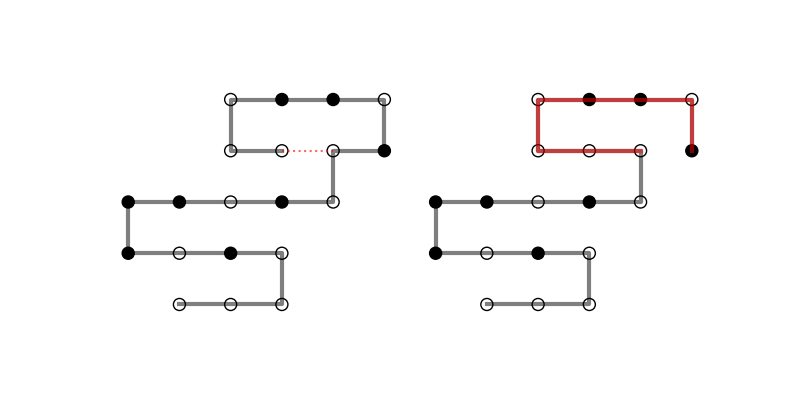
\includegraphics[width=0.45\textwidth]{images/reconnect.png}
	\caption{Пример смены соединений в конфигурации.}
	\label{fig:reconnect}
\end{figure}   

Для  повышения эффективности исследования геометрического состояния алгоритмом, мы также используем методы смены соединений в конфигурации \ref{fig:reconnect}. 

Смена соединений -  это глобальный ход, при котором один участок цепи временно разрывается и пересоединяется в другом месте, сохраняя связность и избегая самопересечений. 

Данная часть алгоритма меняет только соединения в геометрической конфигурации, но не  передвигает узлы и не генерирует новые спиновые состояния. Следовательно, если новое состояние удалось сгенерировать - условия на отсутствие самопересечений не нарушено - оно всегда принимается согласно правилу Метрополиса, так как   $\Delta E = 0 $. 


\begin{figure}
	\centering
	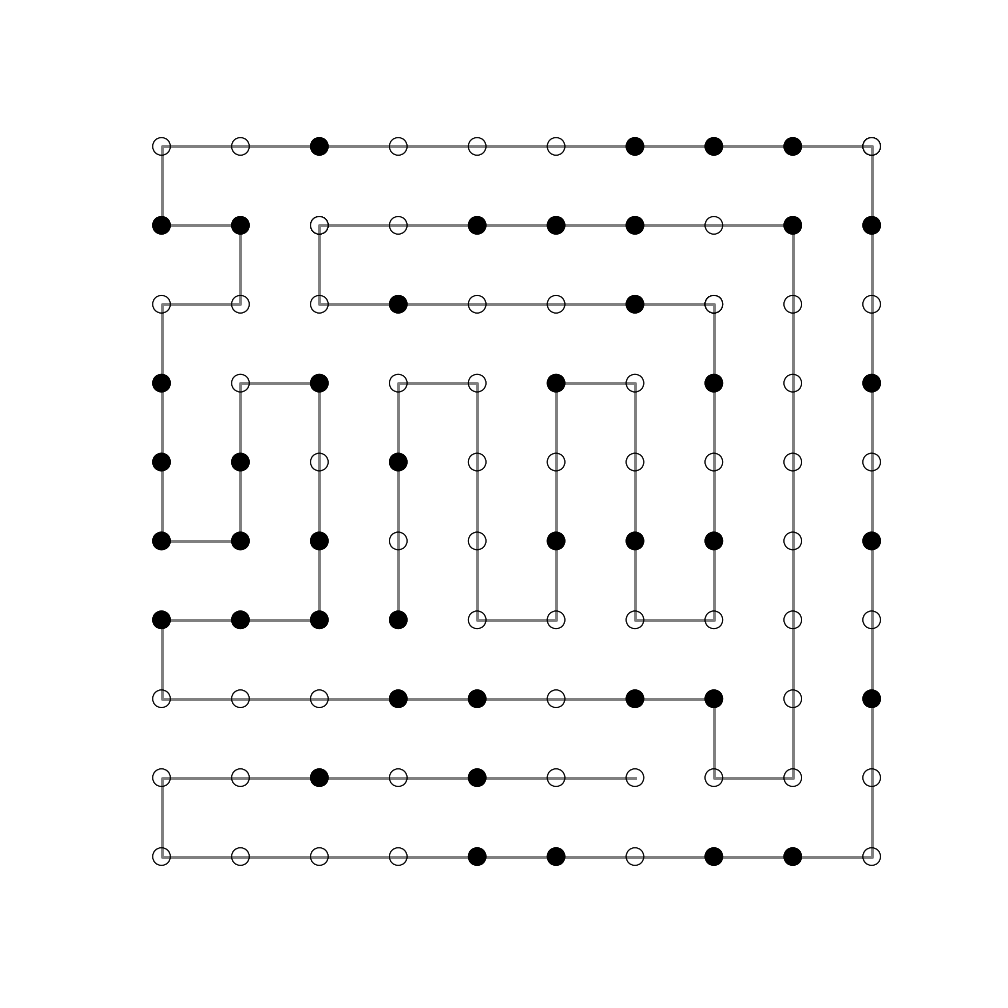
\includegraphics[width=0.35\textwidth]{images/snakeproblem.png}
	\caption{Пример замороженного состояния.}
	\label{fig:reconnect_fix}
\end{figure}   


Такой алгоритм позволяет системе выйти из замороженных состояний  \ref{fig:reconnect_fix}, что делает реализацию алгоритма эргодичной (что не помешает системе, даже если вероятность таких состояний мала). 

 \textbf{Оценка алгоритма}.  
 
  При успешной генерации нового геометрического состояния в среднем меняются соединения   y  $N/2$ узлов в БСП. 
Добавление смены соединений  позволяет  снизить  автокорреляцию  глобальных наблюдаемых примерно на порядок по сравнению с чистым змееподобным‑алгоритмом при сопоставимых суммарных вычислительных затратах.  


\subsection{Кластерная генерация спиновой конфигурации}
%
%

Мы применяем классический алгоритм Вольфа \cite{PhysRevLett.62.361}. Данный алгоритм повыщает эффективность изучения спиновых конфигураций. 

Основная идея алгоритма заключается в формировании кластера $C$ и перевороте его спинов. 
Правила принятия нового состояния должны подчиняться условию детального баланса. 
Мы следуем классическому способу реализации кластерного обновления для модели XY, обсуждаемому в работе \cite{newman1999monte}.


\textbf{Кластерная генерация для XY модели}. 

Перевернуть спин, используя выбранное направление $\vec{n}$, означает изменить знак вектора $ \vec{n} \vec{S_i} (\theta_i) = \vec{n}(\cos \theta_i \sin \theta_i )$ на противоположный. Пример проиллюстрирован на графике \ref{fig:clusterflip}. 


  \begin{figure}
	\centering
	\captionsetup{justification=centering}
	\begin{subfigure}[b]{0.45\textwidth}
		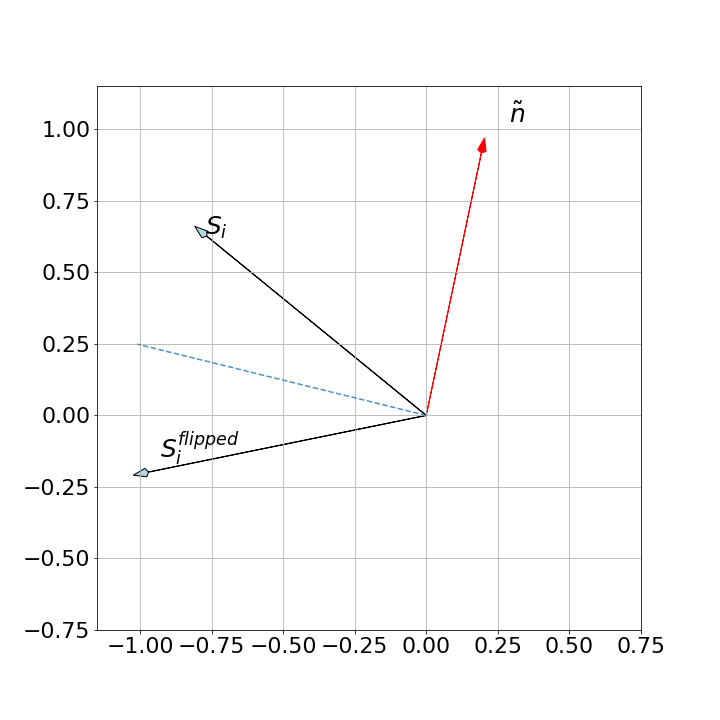
\includegraphics[width=\textwidth]{images/cluster_flip.png}
		\caption{ Пример переворота спина. Сплошная красная стрелка — случайно выбранный единичный вектор $\vec{n}$. Пунктирная синяя линия — перпендикулярная плоскость.}
		\label{fig:clusterflip}
	\end{subfigure}
	\begin{subfigure}[b]{0.45\textwidth}
		\includegraphics[width=\textwidth]{images/state_example_cluster.png}
		\caption{  Пример роста кластера из начальной точки. Синие стрелки показывают направления попыток добавления новых спинов в кластер. Цвет узлов соответствует угловым значениям спинов. }
		\label{fig:clustergrowth}
	\end{subfigure}
	\caption{ Кластерная генерация для XY модели на БСП.  }
	\label{fig:ClusterUpdate}
\end{figure}

Генерация нового состояния с помощью кластерного алгоритма состоит из следующих шагов. 

\begin{enumerate}
	
	\item Случайно выбирается один спин  $\overrightarrow{S_{start}}$, используя  дискретное равномерное распределение (всего $N$ значений, где $N$ --- длина цепочки).
	Мы добавляем этот  спин к кластеру $C$ и отмечаем его как  проверенный.
	Также добавляет этот спин во временный массив $C_{temp}$ для обхода соседей.  
	
	\item Случайно выбирается направление на единичной окружности $\overrightarrow{n}$ с использованием равномерного распределения $ \theta_{new} = U(-\pi, \pi)$: $\overrightarrow{n} = [\cos(\theta_{new}), \sin(\theta_{new})]$.

	\item Берется следующий спин $ \overrightarrow{S_{i}}$  из временного массива $C_{temp}$ , чтобы посетить всех его соседей $S_j$ (  пример обхода соседних узлов показан на графике \ref{fig:clustergrowth} ). 
	Новый спин добавляется в кластер только если проекции спинов на направление $\hat{\mathbf n}$ имеют одинаковый знак, то есть $( \overrightarrow{S_{i}}\overrightarrow{n} )( \overrightarrow{S_{j}}\overrightarrow{n} )>0$. 
	
 Новый спин добавляется в кластер $C$ с вероятностями $P_{add}(\overrightarrow{S_{i}}, \overrightarrow{S_{j}} ) = 1 - \exp \left(-2J (\overrightarrow{S_{i}}\overrightarrow{n})( \overrightarrow{S_{j}} \overrightarrow{n} ) \right)$, где  $\overrightarrow{S_{i}}\overrightarrow{n}$ --- скалярное произведение. 

	
	После посещения всех соседей спина $ \overrightarrow{S_{i}}$,  узел   $ \overrightarrow{S_{i}}$ отмечается как проверенный и  удаляется из временного массива $C_{temp}$.
	
	\item Обход соседей выполняется, пока временный массив $C_{temp}$ не останется пустым. 
	 
	 \item Осуществляется переворот собранного кластера $C$. Спин $\overrightarrow{S_{j}} $ из кластера обновляется через вычитание отраженного вектора: $\overrightarrow{S_{j}} : = \overrightarrow{S_{j}} - 2 \times ( \overrightarrow{S_{j}} \vec{n}) \vec{n}$. 

\end{enumerate}

\textbf{Кластерная генерация для  модели Изинга}. 
 

Для модели Изинга со спинами $s_i \pm1 $ выбор направления не требуется.
Кластер растёт из случайного узла $i_{start}$ так же, как в случае модели XY на БСП, но соседний мономер $j$ добавляется
только если значения спинов  совпадают, $s_i=s_j$, и с вероятностью $P_{\text{add}}(i,j)=1-\exp\!\bigl[-2  J \bigr]$. 
После завершения роста кластера все спины в нём одновременно переворачиваются:
 $ s_i \leftarrow -\,s_i\,,\qquad i\in C$.





 \textbf{Оценка алгоритма}.   
 
 
 Кластерный апдейт строится так, что финальный групповой переворот кластера принимается с вероятностью $1$ (шага Метрополиса  в финале нет). 
 Типичный размер кластера $\langle\lvert C\rvert\rangle$ возрастает при приближении к критической области и может быть порядка $N$ в окрестности критической точки (обсуждения алгоритма в  \cite{newman1999monte}).
 Благодаря этому интегральные автокорреляционные времена, например, для намагниченности и  для энергии, растут существенно медленнее, чем при локальных алгоритмах. 
 


\section{Анализ численных данных}
%
%\subsection{Оценка средних значений : Binning analysis}
%

%Для оценки средних значений и дисперсий автокоррелированных данных, %полученных методом Монте-Карло, мы используем биннинговый (blocking) анализ.
 
 

\subsection{Парная регрессия для оценки точек фазового перехода}


\label{subsection:paired_regression} 
 Мы будем оценивать точки фазовых переходов с помощью метода парных регрессий для  масштабированных кривых радиусов (при изучении структурного перехода) и кумулянтов Биндера  \eqref{binder_cumulant} (при изучении магнитного перехода). 

Основная идея метода --- применение линейной аппроксимации данных, полученных компьютерным  моделированием. 
Метод применяется на наборе данных, срезанных по узкому интервал значений энергии взаимодействия $J \in [J_{min}, J_{max}]$, который покрывает точку фазового перехода. 

Рассмотрим метод парных регрессий для оценки точки магнитного перехода на данных кумулянта Биндера $U_4$. Выберем длину цепочки $N_{fixed}$ для анализа эффекта конечной длины. 

 \begin{enumerate} 
 	
 	\item   Возьмем данные для двух цепочек разной длины $N_{fixed}, N_i$  из узкого диапазона $J \in [J_{min}, J_{max}]$. 
 	\item Для каждой пары значений $N,J$ получим оценку кумулянта Биндера и его ошибку. 
 	
 	\item  Теперь у нас есть две кривые кумулянтов $U_4$ с погрешностями для двух значений $N_{fixed}, N_i$ .  Применим  взвешенную регрессию для двух линий.
 	
	\item   Используя линейную аппроксимацию, найдем точку пересечения двух линий. Это и есть полученная оценка для $\hat{J}$.
 	
  \end{enumerate}

Анализируя все доступные в вычислительных данных пары $N_{fixed}, N_i$, мы получаем зависимость, как оценка критической точки $\hat{J}_{cr}^{fixed}$ зависит от размера парной цепи $N_i$. 
Рассмотрим функцию $\hat{J}^{fixed} = \hat{J}_{cr}^{fixed} (1/N_i)$ и найдём её нулевое значение: $\hat{J}_{cr}^{fixed} (0)$.  
Это значение соответствует термодинамическому пределу  $N_i \rightarrow \infty$.


Повторение парных регрессий и аппроксимация точек пересечения относительно $(1/N_i)$ позволяет нам экстраполировать данные до термодинамического предела.
 Метод позволяет проанализировать, как эти точки пересечения изменяются в зависимости от размера системы и обеспечивает систематический способ анализа эффектов конечного размера.

  
